%%%%%%%%%%%%%%%%%%%%%%%%%%%%%%%%%%%%%%
% TRB Poster 2015
% Created by Subasish Das
% January 2015
%%%%%%%%%%%%%%%%%%%%%%%%%%%%%%%%%%%%%%

\documentclass[final]{beamer}
\usepackage[scale=1.24]{beamerposter}
\usepackage{graphicx}			% allows us to import images

%-----------------------------------------------------------
% Custom commands that I use frequently
%-----------------------------------------------------------

\newcommand{\bb}[1]{\mathbb{#1}}
\newcommand{\cl}[1]{\mathcal{#1}}
\newcommand{\fA}{\mathfrak{A}}
\newcommand{\fB}{\mathfrak{B}}
\newcommand{\Tr}{{\rm Tr}}
\newtheorem{thm}{Theorem}

%-----------------------------------------------------------
% Define the column width and poster size
%-----------------------------------------------------------

\newlength{\sepwid}
\newlength{\onecolwid}
\newlength{\twocolwid}
\setlength{\paperwidth}{48in}
\setlength{\paperheight}{36in}
\setlength{\sepwid}{0.024\paperwidth}
\setlength{\onecolwid}{0.22\paperwidth}
\setlength{\twocolwid}{0.464\paperwidth}
\setlength{\topmargin}{-0.5in}
\usetheme{confposter}
\usepackage{exscale}

%-----------------------------------------------------------
% The next part fixes a problem with figure numbering. Thanks Nishan!
%-----------------------------------------------------------

\usecaptiontemplate{
\small
\structure{\insertcaptionname~\insertcaptionnumber:}
\insertcaption}

%-----------------------------------------------------------
% Define colours (see beamerthemeconfposter.sty to change these colour definitions)
%-----------------------------------------------------------

\setbeamercolor{block title}{fg=Brown,bg=white}
\setbeamercolor{block body}{fg=Black,bg=white}
\setbeamercolor{block alerted title}{fg=white,bg=Sepia!70}
\setbeamercolor{block alerted body}{fg=black,bg=YellowGreen!10}

%-----------------------------------------------------------
% Name and authors of poster/paper/research
%-----------------------------------------------------------

\title{Factor Association Using Multiple Correspondence Analysis in Vehicle-Pedestrian Crashes}
\author{Subasish Das, PhD Candidate \hspace{5in} Xiaoduan Sun, PhD \& PE, Professor}
\institute{University of Louisiana \hspace{10in} University of Louisiana }
%\date{\Large 26 April 2013}

%-----------------------------------------------------------
% Start the poster itself
%-----------------------------------------------------------

\begin{document}
\begin{frame}[t]
  \begin{columns}[t]												% the [t] option aligns the column's content at the top
    \begin{column}{\sepwid}\end{column}			% empty spacer column
    \begin{column}{\onecolwid}
      \begin{alertblock}{Research Question}
        \small{\rmfamily{What are the key contributing factors for vehicle pedestrian crashes? What's the purpose of using multiple correspondence analysis (MCA) in place of conventional parametric approaches?}}
      \end{alertblock}
      \vskip2ex
      \begin{block}{Abstract}
        \small{\rmfamily{This research uses \textbf{Multiple Correspondence Analysis (MCA)}, a data analysis method used for detecting and representing underlying structures in a categorical data set, to analyze eight years (2004-2011) of vehicle-pedestrian crashes in Louisiana. The findings indicated several non-trivial focus groups such as drivers with high occupancy vehicles, female drivers in bad weather conditions, and drivers distracted by mobile phone use. Other key associated factors were hillcrest roadways, dip/hump aligned roadways, roadways with multiple lanes, and roadways with no lighting at night. Male drivers were seen to be more inclined towards severe and moderate injury crashes. Fatal pedestrian crashes were correlated to two-lane roadways with no lighting at night.  This method helped to measure significant contributing factors and degrees of association between the factors by analyzing the systematic patterns of variations with categorical datasets of pedestrian crashes. }}
      \end{block}
      \vskip2ex
      \begin{block}{Introduction}
        \small{\rmfamily{In 2011, 4,432 pedestrians were killed (14\% of total traffic crash fatalities) and 69,000 pedestrians were injured in vehicle-pedestrian crashes in the United States. Improvement of pedestrian safety is one of the topmost priorities in the American Association of State Highway and Transportation (AASHTO) Strategic Highway Safety Plan (SHSP).}}

        \vspace{0.25in}

        \small{\rmfamily{The vehicle-pedestrian crash statistics of Louisiana call for instant and advanced solutions to alleviate safety concerns of the pedestrians. The objective of this study was the application of MCA on vehicle-pedestrian crashes to (1) identify the relative closeness of the key association factors, (2) find important nontrivial association between the key factors and (3) provide intuitions to select better countermeasures to improve pedestrian safety. Improving pedestrian safety is crucial to accomplish the state \textquotesingle s \textbf{Destination Zero Deaths} goal and the MCA method used in this paper will help to find the relative closeness of the key association factors so that necessary actions can be taken to improve the strategy of pedestrian safety.}}

         \vspace{0.25in}

        \small{\rmfamily{The research introduced in this paper is unique and different from previous studies and serves as a starting point to demonstrate the use of MCA to determine the significant cloud of crash contributing factors for vehicle pedestrian crashes which could help state agencies develop the most efficient crash countermeasures.}}

      \end{block}
    \end{column}

    \begin{column}{\sepwid}\end{column}			% empty spacer column
    \begin{column}{\twocolwid}							% create a two-column-wide column and then we will split it up later
      \begin{columns}[t,totalwidth=\twocolwid]	% split up that two-column-wide column
        \begin{column}{\onecolwid}\vspace{-.69in}
          \begin{block}{Multiple Correspondence Analysis}
            \small{\rmfamily{Multiple Correspondence Analysis (MCA) is widely used in categorical data analysis, especially in social science and marketing research, and is considered as an extension of correspondence analysis (CA) to more than two variables. It is an exploratory data analysis method that can visualize the patterns of the cluster consisting of key contributing factors.}}
            \begin{itemize}
              \item For a database with categorical variables, the scheme of the MCA method can be explained by taking an individual row or record \textit{i} as an example where three variables (represented by three columns) have three different category indicators (a1, b1, and c3).
              \item The spatial distribution of the points calculated by the dimensions based on these three categories would be generated by MCA. MCA yields two clouds of points as shown in the figure: the cloud of individual records and the cloud of categories.
              \item A cloud of points is not just a simple "graphical display", it is similar to a geographic map with the same distance scale in all directions.
            \end{itemize}
            \vspace{0.25in}
            \begin{figure}
              \begin{center}
                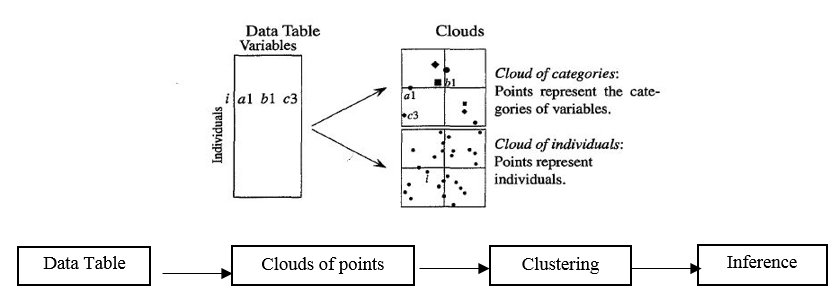
\includegraphics[width=9in, height=2.5in]{A1.png}
                \caption{Clouds of points generated by MCA method.}
                \label{fig:multDom}
              \end{center}
            \end{figure}
          \end{block}
        \end{column}
        \begin{column}{\onecolwid}\vspace{-.69in}
          \begin{block}{Data Description}
             \small{\rmfamily{Eight years (2004-2011) of Louisiana crash data was used in this study. }}
             \begin{itemize}
              \item In the crash database, there are numerous variables that are non-pertinent for this research, such as: the VIN, driver \textquotesingle s license number, database manager \textquotesingle s name, police report number etc. To focus on the meaningful analysis, a set of key variables were selected such as the roadway geometrics (alignment and lighting), collision type, environmental factor (weather), driver related factors (driver gender, age and condition), number of occupants and pedestrian related factor (pedestrian gender, age, condition and severity). The variable section method used the research findings of the previous related research with engineering judgment.
              \item An initial analysis indicated that some variables are highly skewed which means that a majority of crashes fall into one of the two or more categorical values. For example, 94\% of the crashes involved roadways with straight level alignment, 76\% of the crashes were single vehicle crashes, and 78\% of crashes involved single occupant crashes.
              \item It is seen that 61\% of pedestrians involved in crashes were male which was higher than the general trend (around 50 to 55\% of traffic crashes involved male drivers in Louisiana). The not-too-skewed variables include collision type, pedestrian injury, and lighting condition.
            \end{itemize}

          \end{block}
        \end{column}
      \end{columns}
      \vskip2.5ex
      \begin{alertblock}{Major Findings}		% an ACTUAL two-column-wide column
        \small{\rmfamily{The results of the MCA detects several interesting combination clouds. The future work on the degree of association of the crash contributing factors can help safety management systems identify the most effective crash reduction strategies.}}
      \end{alertblock}
      \begin{columns}[t,totalwidth=\twocolwid]
        \begin{column}{\onecolwid}
        \begin{block}{Principle MCA Plot}

            \begin{figure}
              \begin{center}
                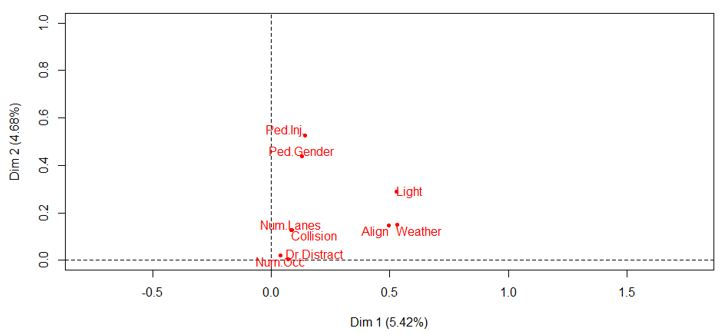
\includegraphics[width=10in, height=3.5in]{m1.jpg}
                %\caption{MCA plot for the variable categories.}
                %\label{fig:multDom}
              \end{center}
            \end{figure}
              \begin{figure}
              \begin{center}
                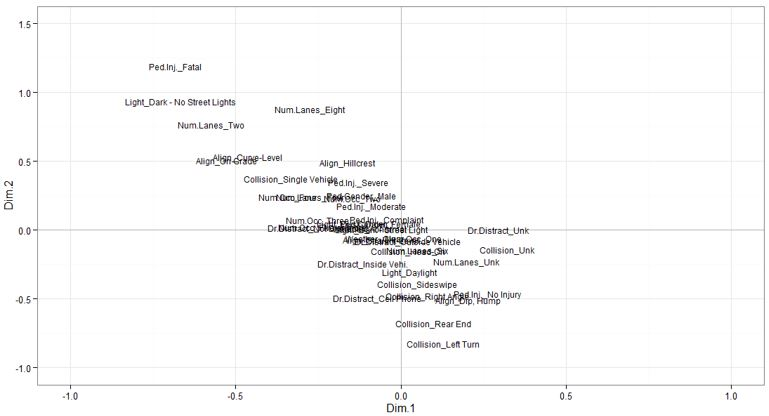
\includegraphics[width=10in, height=3.2in]{m2.jpg}
                \caption{MCA plot for the variable categories.}
                \label{fig:multDom}
              \end{center}
            \end{figure}
        \end{block}
      \end{column}
      \begin{column}{\onecolwid}
        \begin{block}{Combination Clouds}
        \begin{figure}
              \begin{center}
                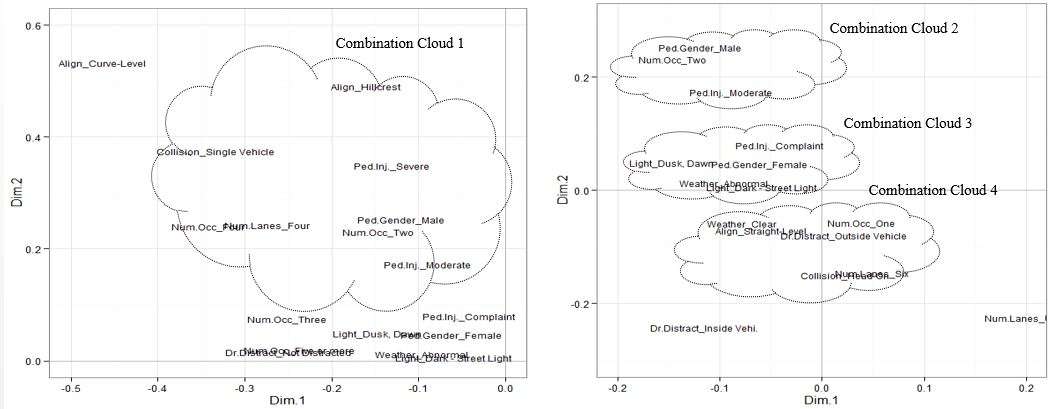
\includegraphics[width=10in, height=3.5in]{m3.jpg}

              \end{center}
            \end{figure}
          \begin{figure}
              \begin{center}
                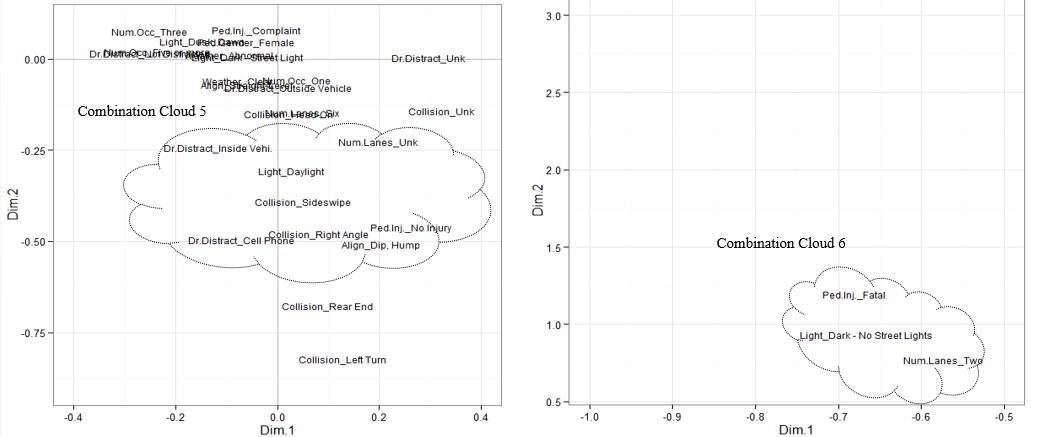
\includegraphics[width=10in, height=3.2in]{m4.jpg}
                \caption{Combination Clouds.}
                \label{fig:multDom}
              \end{center}
            \end{figure}
        \end{block}
      \end{column}
    \end{columns}
  \end{column}
  \begin{column}{\sepwid}\end{column}			% empty spacer column
  \begin{column}{\onecolwid}
    \begin{block}{Discussion}
             \small{\rmfamily{Discussion on the combination clouds are stated below:}}
              \begin{itemize}
              \item \textbf{Combination cloud 1} combines a wider variety of variable categories: hillcrest aligned four-lane roadways, single vehicle collisions, severe and moderate pedestrian injuries, number of occupants 2 and 3, and male pedestrians.  It indicates that hillcrest aligned four-lane roadways were crash prone towards moderate and severe pedestrian injury. It also indicates that larger occupancy vehicles were responsible for single vehicle-pedestrian crashes on this specific type of roadway.
              \item \textbf{Combination cloud 2} associates male pedestrians with moderate injury crashes while the number of occupants in the vehicles was two.  It indicates that car occupancy had some role in pedestrian related crashes.
              \item \textbf{Combination cloud 3} associated several factors: complaint injury of female pedestrians, dawn or dusk, abnormal weather and night time crashes in roadways with lighting. \textbf{Combination cloud 4} combines a few factors: clear weather, single occupant, six-lane straight-level aligned roadways, head-on collisions and driver distraction due to outside events. Both of the findings are non-trivial in nature.
              \item \textbf{Combination cloud 5} also associates different variable categories: driver distraction from mobile or inside equipment, daytime right angle and sideswipe crashes, dip/hump roadways with unknown information on lanes, and PDO pedestrian crashes. This combination indicates cell phone involvement in dip/hump aligned roadways.
              \item \textbf{Combination cloud 6} associates three variable categories: fatal pedestrian crash, nighttime crash, and two-lane roadways with no lighting. It indicates that absence of lighting at night is a significant factor for pedestrian traffic severity. This cloud clearly indicates one major focus group on roadway geometrics.
            \end{itemize}
            \end{block}
    \vskip2ex


    \begin{block}{Conclusion}
        \small{\rmfamily{In particular the ability of MCA to deal with multidimensional data makes it particularly useful for exploring the factors influencing traffic crash occurrences. The findings from this research shed light on the pattern recognition of vehicle-pedestrian crashes and expose new aspects in pedestrian safety and also point to potential future research considering more variables and large dataset from multiple states. }}
     \vspace{0.35in}


      \begin{center}
        \begin{tabular}{ccc}
          
\includegraphics[width=3in, height=3in]{ulls.jpg}
        \end{tabular}
      \end{center}
    \end{block}
  \end{column}
  \begin{column}{\sepwid}\end{column}			% empty spacer column
 \end{columns}
\end{frame}
\end{document}
